\documentclass[11pt,a4paper]{article}

\usepackage{../../templates/style}

\begin{document}

\begin{problem}{Seven Segment}{standard input}{standard output}{1 second}{64 megabytes}

ระบบแสดงผลตัวเลขแบบเจ็ดส่วน เป็นระบบแสดงผลที่นิยมใช้กันมากในอุปกรณ์ไฟฟ้าหลายอย่าง เช่นเป็นตัวเลขบอกชั้นสำหรับลิฟต์ เป็นระบบแสดงผลของนาฬิกาดิจิตอล และเป็นระบบแสดงผลเครื่องมือวัดหลายชนิด สมมุติว่ามีระบบเก็บภาพจากระบบแสดงตัวเลขแบบเจ็ดส่วนด้วยเมตริกซ์ขนาด $3 \times  3$ และใช้ตัวอักขระ $3$ ตัวที่อยู่บนแป้นพิมพ์เท่านั้น คือ \textbf{เว้นวรรค ' ' (Space bar) , ตัวขีดล่าง ‘\_’ (Underscore) }และ\textbf{เส้นดิ่ง ‘|’ (Vertical bar)} แทนแต่ละส่วนของตัวเลขแบบเจ็ดส่วนคือ เว้นวรรค แทนการไม่มีส่วนของตัวเลขในช่องนั้น ตัวขีดล่างแทนส่วนของตัวเลขตามแนวนอน และเส้นดิ่งแทนส่วนของตัวเลขตามแนวดิ่งดังภาพ


\begin{figure}[h]
\centering
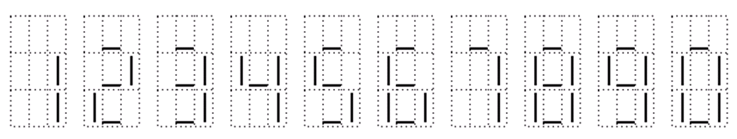
\includegraphics[width=0.8\textwidth]{../latex/img/1009/1009-1.png}
\caption{ระบบแสดงเลขแต่ละตัวตั้งแต่ 0 ถึง 9 โดยการใช้ตัวอักขระ}
\end{figure}

\underline{\textbf{โจทย์}} จงเขียนโปรแกรมเพื่ออ่านรูปแบบข้อมูลของระบบแสดงผลตัวเลขแบบเจ็ดส่วนตามรูปแบบที่กำหนดสองชุด ทำการแปลงเป็นจำนวนเต็มสองจำนวน หาผลบวกของตัวเลขสองจำนวนนั้น และแสดงค่าผลบวกที่ได้

\InputFile

\textbf{บรรทัดแรก} รับจำนวนเต็มบวก $A$ $B$ (คั่นด้วยเว้นวรรค $1$) วรรคแทนจำนวนหลักของตัวเลขชุดแรกและชุดที่สองตามลำดับ โดยที่ $1 \leq A,B \leq 10$ 

\textbf{บรรทัดที่สองถึงสี่} รับข้อมูลเป็นรูปแบบแสดงผลตัวเลขแบบเจ็ดส่วนของตัวเลขชุดแรกทั้งหมด $A$ หลัก และแต่ละหลักคั่นด้วยเว้นวรรคจำนวน $1$ วรรค 

\textbf{บรรทัดที่ห้าถึงเจ็ด} รับข้อมูลเป็นรูปแบบแสดงผลตัวเลขแบบเจ็ดส่วนของตัวเลขชุดที่สองทั้งหมด $ฺB$ หลัก และแต่ละหลักคั่นด้วยเว้นวรรคจำนวน $1$ วรรค 

\OutputFile

\textbf{มีบรรทัดเดียว} แสดงค่าจำนวนเต็มค่าเดียว เป็นผลบวกของจำนวนเต็มสองจำนวนที่เป็นข้อมูลนำเข้า รับประกันว่าค่านี้เป็นจำนวนเต็มบวกที่มีค่าไม่เกิน $2^{32} – 1$

\Examples

\begin{example}
\exmp{4 2
\text{               }
\text{  | |\_|   | |\_|}
\text{  |   |   |   |}
\text{       }
\text{|\_|   |}
\text{  |   |}}{1455}%
\exmp{4 3
\text{         \_   \_ }
\text{  | |\_|  \_|  \_|}
\text{  |   | |\_   \_|}
\text{ \_       \_ }
\text{  |   | |\_ }
\text{  |   | |\_|}}{2139}%
\end{example}

\Source

การแข่งขันคอมพิวเตอร์โอลิมปิก สอวน. ครั้งที่ 2 มหาวิทยาลัยบูรพา

\end{problem}

\end{document}